\documentclass[a4paper, 12pt]{article}
\usepackage[a4paper,top=1.5cm, bottom=1.5cm, left=1cm, right=1cm]{geometry}
\usepackage{cmap}					% поиск в PDF
\usepackage{mathtext} 				% русские буквы в формулах
\usepackage[T2A]{fontenc}			% кодировка
\usepackage[utf8]{inputenc}			% кодировка исходного текста
\usepackage[english,russian]{babel}	% локализация и переносы

\usepackage{amsmath}
\usepackage{indentfirst}
\usepackage{longtable}
\usepackage{graphicx}
\usepackage{array}

\usepackage{wrapfig}
\usepackage{siunitx} % Required for alignment
\usepackage{subfigure}
\usepackage{multirow}
\usepackage{rotating}
\usepackage{caption}

\graphicspath{{.}}


\title{\begin{center}Лабораторная работа №2.1.2\end{center}
Определение $C_p / C_v$ методом адиабатического расширения}
\author{Рожков А. В. \\ Преподаватель Яворский В. А.}
\date{\today}

\begin{document}
    \pagenumbering{gobble}
    \maketitle
    \newpage
    \pagenumbering{arabic}

    \textbf{Цель работы:} определение отношения $C_p / C_v$ углекислого газа  по измерения давления в стеклянном сосуде. Измерения производятся сначала после адиабатического расширения газа а затем после нагревания сосуда и газа до комнатной температуры.

	\textbf{В работе используются:} стеклянный сосуд: U-образный жидкостный манометр; резиновая груша; газгольдер с углекислым газом.

	\begin{figure}[b!]	\label{plan2}

		\center{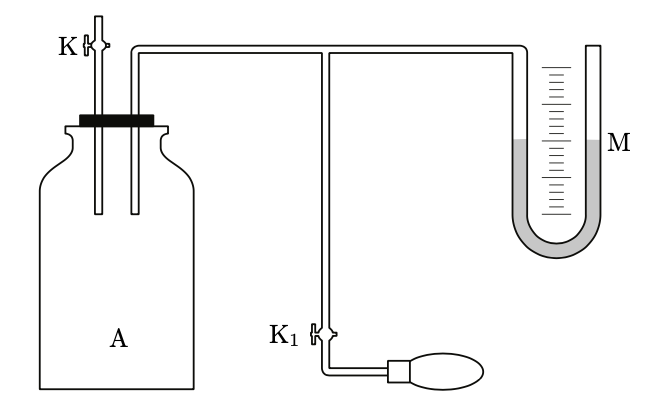
\includegraphics[width=1 \linewidth]{img/ust.jpg}}
		\caption{Установка для определения $C_p / C_v$ методом адиабатического расширения газа}

	\end{figure}

	\section{Экспериментальная установка}

		Используемая для опытов экспериментальная установка состоит из стеклянного сосуда А (объёмом около 20 л), снабженного краном К, и U-образного жидкостного манометра, измеряющего избыточное давление газа в сосуде. Схема установки показана на Рис. 1.

		Избыточное давление создаётся с помощью резиновой груши, соединённой с сосудом трубкой с краном $К_1$.

		В начале опыта  в стеклянном сосуде А находится исследуемый газ при комнатной температуре $T_1$ и давлении $P_1$, несколько превышающем атмосферное давление  $P_0$. После открытия крана К, соединяющего сосуд А с атмосферой, давление и температура газа будут понижаться. Это уменьшение температуры приближённо можно считать адиабатическим.

		Для адиабатического процесса можно записать следующее уравнение:

		\begin{equation}\label{mk}
		\left(\dfrac{P_1}{P_2}\right)^{\gamma - 1} = \left(\dfrac{T_1}{T_2}\right)^\gamma ,
		\end{equation}

		где индексом "1" обозначено состояние после повышения давления в сосуде и выравнивания температуры с комнатной, а индексом "2"  $-$ сразу после открытия крана и выравнивания давления с атмосферным.

		После того, как кран К вновь отсоединит сосуд от атмосферы , происходит медленное изохорическое нагревание газа со скоростью, определяемой теплопроводностью стеклянных стенок сосуда. Вместе с ростом температуры растёт и давление газа. З время порядка $\Delta t_T$  (время установления температуры) система достигает равновесия, и установившаяся температура газа $T_3$ становится равной комнатной температуре $T_1$.

		Тогда используя закон Гей-Люссака для изохорического процесса и уравнение \eqref{mk} найдём $\gamma$:

		\begin{equation}\label{acc}
		\gamma = \dfrac{\ln(P_1 / P_0)}{\ln (P_1 / P_3)}.
		\end{equation}

		С учётом того, что $P_i = P_0 + \rho g h_i$ и пренебрегая членами второго порядка малости получим из \eqref{acc}:

		\begin{equation}\label{r}
		\gamma \approx \dfrac{h_1}{h_1 - h_2}.
		\end{equation}


\end{document}
